\documentclass[conference]{IEEEtran}
\IEEEoverridecommandlockouts
% The preceding line is only needed to identify funding in the first footnote. If that is unneeded, please comment it out.
\usepackage{cite}
\usepackage{amsmath,amssymb,amsfonts}
\usepackage{algorithmic}
\usepackage{graphicx}
\usepackage{textcomp}
\usepackage{xcolor}
\def\BibTeX{{\rm B\kern-.05em{\sc i\kern-.025em b}\kern-.08em
    T\kern-.1667em\lower.7ex\hbox{E}\kern-.125emX}}
\begin{document}

\title{PryGuard Browser: Enhancing Online Privacy with Advanced Anti-Fingerprinting, Cookie Containerization, and Temporary Email Generation\\
% {\footnotesize \textsuperscript{*}Volume 1, No 1}

}

\author{
\IEEEauthorblockN{Pannag Kumaar}
\IEEEauthorblockA{\textit{Department of Computer Science} \\
\textit{PES University}\\
Bangalore, India \\
pannag2003@gmail.com}
\and
\IEEEauthorblockN{Maryam Khan}
\IEEEauthorblockA{\textit{Department of Computer Science} \\
\textit{PES University}\\
Bangalore, India \\
kmaryam@gmail.com}
\and
\IEEEauthorblockN{N Tania Somanna}
\IEEEauthorblockA{\textit{Department of Computer Science} \\
\textit{PES University}\\
Bangalore, India \\
tania.somanna@gmail.com}
\and
\IEEEauthorblockN{\hspace{4cm}Himank Bansal}
\IEEEauthorblockA{\textit{\hspace{4cm}Department of Computer Science} \\
\textit{\hspace{4cm}PES University}\\
\hspace{4cm}Bangalore, India \\
\hspace{4cm}b.himank101@gmail.com}
\and
\IEEEauthorblockN{\hspace{-2cm}Sarasvathi V}
\IEEEauthorblockA{\textit{\hspace{-2cm}Department of Computer Science} \\
\textit{\hspace{-2cm}PES University}\\
\hspace{-2cm}Bangalore, India \\
\hspace{-2cm}Sarsvathiv@pes.edu}
}


}

\maketitle

\begin{abstract}
Modern web tracking mechanisms rely heavily on browser fingerprinting, cross-site tracking, and persistent cookies to build unique user profiles. Traditional privacy measures are inadequate against these advanced techniques. This paper presents a multi-faceted approach combining dynamic JavaScript overrides for anti-fingerprinting, per-profile cookie containerization, and temporary email generation. These methods collectively enhance anonymity by injecting randomized data into browser attributes, isolating cookies within user profiles, and offering disposable email addresses. The proposed techniques significantly outperform existing solutions, ensuring robust privacy without sacrificing usability.
\end{abstract}

\begin{IEEEkeywords}
Anti-Fingerprinting, Obfuscation with Randomized Fingerprints, Proxy Management, Cookie Containerization, Temporary Email Generation, Cloudflare API, Online Privacy, MVVM Architecture, WPF, Chromium Embedded Framework

\end{IEEEkeywords}

\section{Introduction}
The growing sophistication of web tracking technologies has heightened the importance of privacy-preserving mechanisms in modern browsers. Browser fingerprinting is one of the most insidious methods used by trackers, relying on subtle variations in browser APIs, hardware configurations, and user behaviors to uniquely identify individuals. Complementary techniques, such as cross-site tracking via cookies and email-based profiling, amplify these threats by enabling persistent user monitoring across multiple domains and sessions. These tracking techniques can collect a wide range of user data, from browsing habits to system configurations, which can be used to build detailed profiles that compromise user anonymity.

Existing solutions such as Tor Browser and Firefox’s Enhanced Tracking Protection provide partial mitigation. Tor Browser anonymizes traffic but often imposes usability constraints by requiring frequent session resets. Similarly, Firefox limits third-party tracking through cookie management but lacks comprehensive anti-fingerprinting capabilities. Chrome’s focus on cookie partitioning overlooks vulnerabilities in JavaScript-based fingerprinting and hardware attribute spoofing. These limitations underscore the need for a comprehensive framework that integrates robust anti-fingerprinting, granular cookie management, and email anonymization into a cohesive privacy-preserving solution.

The proposed framework dynamically overrides JavaScript APIs to inject randomized anti-fingerprinting attributes, creates per-profile cookie containers to prevent cross-site data leakage, and leverages temporary email generation to anonymize online communications. This paper evaluates the efficacy of these techniques against modern tracking mechanisms and demonstrates their superiority in maintaining user privacy.

The presented framework combines dynamic anti-fingerprinting, cookie containerization, and temporary email generation to address key vulnerabilities in user privacy. These features work cohesively to create a robust defense against tracking mechanisms:

\begin{itemize}
    \item Dynamic Anti-Fingerprinting: This feature dynamically modifies browser APIs during page rendering, injecting randomized attributes to thwart fingerprinting attempts. It covers a wide range of APIs, including WebGL, canvas, audio contexts, WebRTC, and media devices, ensuring comprehensive protection.
    \item Proxy integration offering users IP masking and the ability to switch between multiple proxy settings for enhanced anonymity.
    \item Per-Profile Cookie Containerization: Cookies are isolated into distinct containers for each browsing profile, preventing cross-site data leakage while maintaining session persistence. This approach ensures that cookies from one domain cannot interact with or access data from another, even within the same session.
    \item Temporary Email Generation: The framework automates the creation of disposable email addresses tied to user profiles. These emails enable anonymous registrations and interactions, protecting users from spam, phishing, and email-based tracking.



\end{itemize}
% Windows Presentation Foundation (WPF) and the Model-View-ViewModel (MVVM) architecture is used to build PryGuard, ensuring scalability, maintainability, and separation of concerns. CEFSharp (Chromium Embedded Framework) for rendering web pages ensures high compatibility with modern web technologies while allowing deep integration of privacy-enhancing features.

% By leveraging a combination of anti-fingerprinting, cookie isolation, proxy management, and temporary email services, PryGuard provides a comprehensive solution to modern tracking challenges, without sacrificing usability or browsing experience. Through extensive testing and benchmarking against existing browsers, PryGuard demonstrates how modern privacy-focused browsers can evolve to meet the demands of a surveillance-heavy digital landscape.


\section{Literature Review}

% \subsection{Maintaining the Integrity of the Specifications}

\subsection{Anti-Fingerprinting}
Browser fingerprinting has become a dominant technique for online tracking due to its ability to uniquely identify users based on browser and device attributes. Studies by Laperdrix et al. (2020) [1] demonstrate the extensive use of multimedia APIs, such as WebGL and Canvas, along with hardware attributes, to create persistent identifiers that are difficult to circumvent. While solutions like Firefox’s Enhanced Tracking Protection attempt to address this issue by normalizing certain browser attributes, they often fall short against adaptive trackers. Ajay and Guptha (2022) [3] proposed API normalization techniques, which mask specific browser properties but do not fully counter advanced methods, such as audio context exploitation or WebRTC IP leakage.
Existing tools, such as Tor Browser, provide anonymity by routing traffic through the Tor network and allowing users to change their IP addresses dynamically. However, Tor’s reliance on identity rotation disrupts session continuity and fails to provide customizable fingerprint attributes. Recent advancements have focused on dynamic fingerprinting resistance, where runtime randomization ensures unpredictability. This technique, seen in frameworks like PryGuard, extends protections to a wider range of APIs, including WebRTC and media devices, ensuring comprehensive coverage.

\subsection{Cookie Containerization}
Cookies are critical to the operation of modern websites but also serve as a primary mechanism for cross-site tracking. Research on browser privacy frameworks highlights the limitations of traditional cookie management strategies, such as blocking third-party cookies or partitioning cookies by domain. These methods fail to isolate first-party cookies, which can still be used for tracking across multiple sessions and websites [1][2].

Recent developments emphasize per-profile cookie isolation as an effective strategy to address these limitations. This approach ensures that cookies created during one browsing session are restricted to that session or profile, preventing leakage of data across domains. For example, Google Chrome’s partitioned cookie framework addresses third-party tracking but does not isolate first-party cookies within user profiles [3].

% PryGuard adopts a more granular method by assigning unique cookie containers to individual profiles. This design not only isolates cookies but also allows users to define custom policies, such as expiration times and access permissions, enhancing privacy without disrupting usability. Such measures align with the broader trend of balancing user experience with robust privacy controls.

\subsection{Temporary Email Generation}
Temporary email services have gained traction as an essential tool for preserving user anonymity during online registrations. Platforms like GuerrillaMail and Mailnesia have demonstrated the effectiveness of disposable email addresses in preventing spam and email-based tracking. However, these standalone solutions are often inconvenient and lack integration with broader privacy workflows [1] [2].

Research by Hu et al. (2019) [2] and other scholars explored advanced techniques in temporary email generation, emphasizing the role of automation in enhancing usability. For instance, systems leveraging natural language processing (NLP) and deep learning have been proposed to create dynamic, anonymized email templates that can scale with user demand [8].

Building on this foundation, PryGuard integrates temporary email generation directly into its privacy framework. By associating email aliases with user profiles, it enables seamless online interactions while protecting users from spam and phishing attacks. This integrated approach provides a significant improvement over existing services by combining scalability with anonymity.





% Over the years, several browsers have attempted to address privacy concerns, particularly those related to tracking and online anonymity. While some of these browsers provide basic mechanisms to block cookies and  third-party trackers, they are ineffective at completely addressing more advanced techniques like browser fingerprinting.

% Firefox's Fingerprinting Protection: Firefox’s claim to provide complete protection through its Enhanced Tracking Protection extension falls short in practice. Despite enabling some level of fingerprinting resistance, the functionality is often patchy. This limitation leaves users exposed to certain advanced fingerprinting techniques that PryGuard addresses by allowing custom fingerprint injection, ensuring better anonymization and resistance to tracking .

% Tor Browser Identity Change: Tor offers a powerful tool for anonymity, allowing users to change their identity by switching IP addresses through the Tor network. However, this feature does not permit persistent sessions, which leads to usability challenges when users need session continuity. PryGuard overcomes this by supporting seamless profile transitions without sacrificing anonymity or usability .

% Google's Anti-Tracking Mechanisms: Google Chrome offers an option to block third-party cookies, but this blanket approach has limitations. It can break functionality on certain websites while failing to address the more sophisticated tracking mechanisms used by websites today. PryGuard’s cookie containerization offers a refined solution, isolating cookies by profile and allowing users to prevent leakage cookies between profiles .

% Multiple research papers have addressed the challenges of fingerprinting and tracking. Laperdrix et al. (2020) [1] conducted a comprehensive survey of fingerprinting techniques, identifying how browser extensions, multimedia APIs, and JavaScript are exploited for tracking. Hu et al. (2019) [2] explored how disposable email services are leveraged for pixel tracking, which informed the development of PryGuard’s temporary email service to counteract this vulnerability. Ajay and Guptha (2022) [3] introduced API normalization to mask browser attributes, which provided inspiration for PryGuard’s fingerprint injection strategy . However, their solution only addressed JavaScript-based fingerprinting. 

% PryGuard leverages generalized-randomization to craft diverse fingerprint profiles for techniques such as canvas fingerprinting, WebRTC IP leak prevention, and hardware profile injection. PryGuard containerises profiles to prevent leaking of cookies between profiles as well as temporary email generation to maintain user anonymity.



\section{Proposed Methodology}
The framework is developed using Windows Presentation Foundation (WPF) and the Model-View-ViewModel (MVVM) architecture. WPF facilitates the creation of a rich, user-friendly interface while maintaining scalability and extensibility. The MVVM architecture ensures a clear separation of concerns, enhancing maintainability and testability. These architectural choices make the framework adaptable to evolving requirements and capable of integrating new features with minimal disruption.

\begin{figure}[htbp]
\centerline{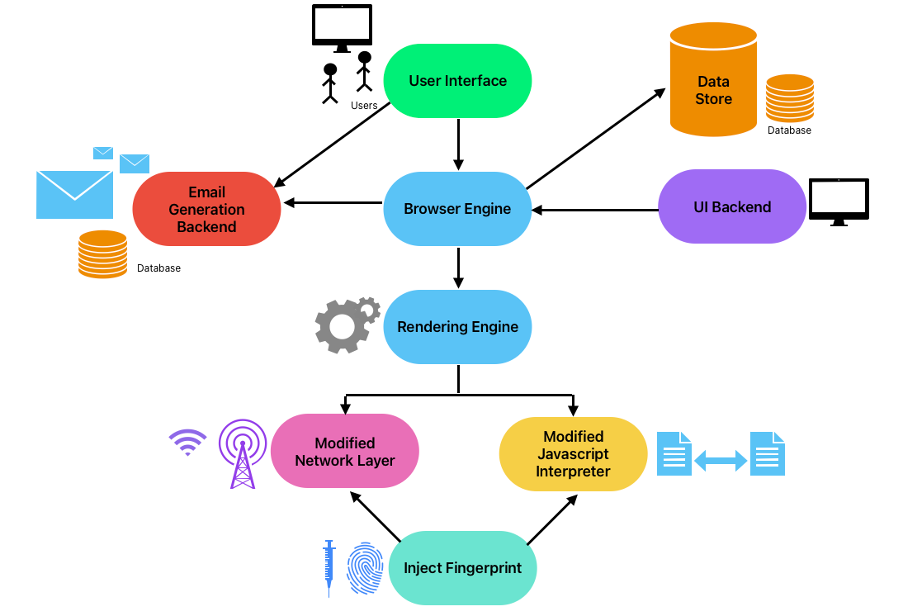
\includegraphics[width=1\linewidth]{HighLevelArch.png}}
\caption{High Level Architecture}
\label{fig}
\end{figure}

For rendering web pages, the framework employs CEFSharp, which is based on the Chromium Embedded Framework (CEF). CEFSharp provides high compatibility with modern web technologies, ensuring that users can access web applications seamlessly. Its integration capabilities allow deep embedding of privacy-enhancing features, such as API spoofing, cookie isolation, and email management, directly within the browser’s runtime environment.

The modular design of the framework allows for independent development and testing of core components. The anti-fingerprinting module dynamically patches JavaScript functions using injected scripts, while the cookie containerization module manages isolated storage for cookies and session data. The temporary email generation module interacts with Cloudflare APIs to create and route disposable emails in real time.

\subsection{Dynamic JavaScript Overrides for Anti-Fingerprinting}
The proposed anti-fingerprinting methodology leverages real-time interception and modification of browser API calls to inject randomized attributes. Unlike static masking, which uses fixed values, this approach ensures that data remains dynamic and unpredictable. For instance, WebGL vendor and renderer strings, often used to identify a user’s hardware, are replaced with randomized values during page rendering. This dynamic injection obfuscates hardware-specific details while maintaining compatibility with legitimate graphical applications.

Similarly, techniques such as Canvas obfuscation are employed to modify pixel-level rendering outputs dynamically, ensuring unique fingerprints for every session without degrading the user experience. Audio fingerprinting, another vector for tracking, is mitigated by introducing subtle noise. These changes preserve the audio functionality of web applications while preventing audio-based fingerprinting.

WebRTC IP masking is implemented by replacing real IP addresses in ICE candidates with dynamically generated values. This approach eliminates the risk of IP leakage during peer-to-peer connections, a common vulnerability in WebRTC-based communications. Media device spoofing extends the protection further by returning randomized attributes from a list of devices. This technique masks hardware capabilities and ensures that trackers cannot rely on static device information.

The framework includes a proxy integration module that supports multiple proxy types, including HTTP, SOCKS4, and SOCKS5. By routing all traffic through a proxy server, the user’s IP address is masked, further enhancing anonymity.

The methodology also includes the dynamic randomization of user-agent strings, ensuring that trackers cannot exploit predictable patterns. By integrating these techniques, the framework ensures that anti-fingerprinting measures apply consistently across all embedded components, eliminating discrepancies that trackers might exploit.

\subsection{Cookie Containerization for Profile-Based Isolation}
The cookie containerization methodology focuses on isolating cookies at the profile level, ensuring that data from one session or website remains inaccessible to others. This isolation is achieved by assigning a unique cookie container to each user profile, effectively preventing cross-site tracking. For example, when a user accesses multiple websites within the same browsing session, cookies from one domain cannot interact with or access data from another.

Custom cookie policies enhance user control by allowing specific configurations for each profile. These policies can include defining expiration times, blocking third-party cookies, or restricting cookie access based on predefined criteria. The framework ensures that cookies persist within individual profiles, enabling seamless session functionality while preventing data leakage.

The methodology supports various use cases, such as accessing sensitive accounts in separate profiles or isolating cookies from tracking-heavy websites. By preventing cookie leakage and cross-domain access, the approach provides a significant advantage over traditional cookie management techniques.

\subsection{Temporary Email Generation for Anonymous Interactions}
Temporary email generation addresses the challenge of email-based tracking and spam by automating the creation of disposable email addresses. Using APIs such as Cloudflare, the framework dynamically generates email aliases tied to user profiles. These temporary addresses are routed to the user’s primary inbox and can be deleted after use, ensuring anonymity during online registrations.

To prevent misuse, the system enforces limits on the number of active temporary emails per profile and requires user verification for email routing. By linking temporary emails to browsing profiles, the framework integrates seamlessly with user workflows, enabling secure and anonymous interactions across websites.















% I. Introduction
% The growing sophistication of web tracking technologies has heightened the importance of privacy-preserving mechanisms in modern browsers. Browser fingerprinting is one of the most insidious methods used by trackers, relying on subtle variations in browser APIs, hardware configurations, and user behaviors to uniquely identify individuals. Complementary techniques, such as cross-site tracking via cookies and email-based profiling, amplify these threats by enabling persistent user monitoring across multiple domains and sessions.

% Existing solutions such as Tor Browser and Firefox’s Enhanced Tracking Protection provide partial mitigation. Tor Browser anonymizes traffic but often imposes usability constraints by requiring frequent session resets. Similarly, Firefox limits third-party tracking through cookie management but lacks comprehensive anti-fingerprinting capabilities. Chrome’s focus on cookie partitioning overlooks vulnerabilities in JavaScript-based fingerprinting and hardware attribute spoofing. These limitations underscore the need for a comprehensive framework that integrates robust anti-fingerprinting, granular cookie management, and email anonymization into a cohesive privacy-preserving solution.

% The proposed framework dynamically overrides JavaScript APIs to inject randomized anti-fingerprinting attributes, creates per-profile cookie containers to prevent cross-site data leakage, and leverages temporary email generation to anonymize online communications. This paper evaluates the efficacy of these techniques against modern tracking mechanisms and demonstrates their superiority in maintaining user privacy.

% II. Existing Privacy Mechanisms and Challenges
% Browser fingerprinting relies on combining various browser, hardware, and software attributes to generate unique identifiers. Attributes such as WebGL vendor strings, canvas rendering data, and audio processing characteristics are often exploited to create highly consistent fingerprints. Current anti-fingerprinting tools primarily use static or partially randomized attributes, which provide limited protection against sophisticated tracking systems capable of identifying patterns over time. Additionally, most existing tools fail to extend their protection to iframe content and other embedded components, leaving significant gaps.

% Cookies remain one of the most widely used mechanisms for persistent tracking. While many browsers now block third-party cookies by default, first-party cookies still allow trackers to correlate user activity across sessions. Modern browsers, including Chrome, offer cookie partitioning, but this approach does not fully isolate cookies at the profile or session level.

% Temporary email systems, such as Mailinator or 10MinuteMail, provide disposable addresses for anonymous registration but often operate as standalone services. These systems lack seamless integration with user workflows and are susceptible to misuse or spam if not managed effectively.

% III. Methodologies
% A. Dynamic JavaScript Overrides for Anti-Fingerprinting
% The proposed anti-fingerprinting methodology leverages real-time interception and modification of browser API calls to inject randomized attributes. Unlike static masking, which uses fixed values, this approach ensures that data remains dynamic and unpredictable. For instance, WebGL vendor and renderer strings, often used to identify a user’s hardware, are replaced with randomized values during page rendering. This dynamic injection obfuscates hardware-specific details while maintaining compatibility with legitimate graphical applications.

% Similarly, canvas fingerprinting, which relies on unique graphical outputs, is countered by modifying the toDataURL method to include randomized noise. The randomness ensures that every session produces unique canvas outputs, effectively nullifying fingerprint consistency. Audio fingerprinting, another vector for tracking, is mitigated by introducing subtle noise into methods like getChannelData and getFloatFrequencyData. These changes preserve the audio functionality of web applications while preventing audio-based fingerprinting.

% WebRTC IP masking is implemented by replacing real IP addresses in ICE candidates with dynamically generated values. This approach eliminates the risk of IP leakage during peer-to-peer connections, a common vulnerability in WebRTC-based communications. Media device spoofing extends the protection further by returning randomized attributes for devices listed via navigator.mediaDevices.enumerateDevices. This technique masks hardware capabilities and ensures that trackers cannot rely on static device information.

% The methodology also includes the dynamic randomization of user-agent strings, ensuring that trackers cannot exploit predictable patterns. By integrating these techniques with iframe content, the framework ensures that anti-fingerprinting measures apply consistently across all embedded components, eliminating discrepancies that trackers might exploit.

% B. Cookie Containerization for Profile-Based Isolation
% The cookie containerization methodology focuses on isolating cookies at the profile level, ensuring that data from one session or website remains inaccessible to others. This isolation is achieved by assigning a unique cookie container to each user profile, effectively preventing cross-site tracking. For example, when a user accesses multiple websites within the same browsing session, cookies from one domain cannot interact with or access data from another.

% Custom cookie policies enhance user control by allowing specific configurations for each profile. These policies can include defining expiration times, blocking third-party cookies, or restricting cookie access based on predefined criteria. The framework ensures that cookies persist within individual profiles, enabling seamless session functionality while preventing data leakage.

% The methodology supports various use cases, such as accessing sensitive accounts in separate profiles or isolating cookies from tracking-heavy websites. By preventing cookie leakage and cross-domain access, the approach provides a significant advantage over traditional cookie management techniques.

% \subsection{Temporary Email Generation for Anonymous Interactions}
% Temporary email generation addresses the challenge of email-based tracking and spam by automating the creation of disposable email addresses. Using APIs such as Cloudflare, the framework dynamically generates email aliases tied to user profiles. These temporary addresses are routed to the user’s primary inbox and can be deleted after use, ensuring anonymity during online registrations.

% To prevent misuse, the system enforces limits on the number of active temporary emails per profile and requires user verification for email routing. By linking temporary emails to browsing profiles, the framework integrates seamlessly with user workflows, enabling secure and anonymous interactions across websites.











% PryGuard’s architecture prioritizes user privacy and flexibility, structured across three main components: Fingerprinting Prevention, Cookie Containerization, and Temporary Email Generation. Each component functions within a modular system that combines the User Interface (UI), Privacy Layer, and Backend Services. Additional features like Developer Tools, Browser UI (with Search History, Downloads, Bookmarks), and Themes further enhance user experience.

% \textbf{Fig 1 }represents our privacy-focused web browser that is built to use a User Profiling Module that protects user privacy by injecting fake fingerprints into the browser's rendering pipeline. This module is used to obfuscate the user's real identity and browsing behavior. It is a deception technique to ward off potential tracking mechanisms and fingerprinting techniques employed by websites or third-party scripts. This privacy-centric browser is designed to prioritize user anonymity and data protection. It comprises the User Interface, Browser Engine, Rendering Engine, Email Generation and Backend Services which are seamlessly integrated together to create our browser.

% \begin{figure}[htbp]
% \centerline{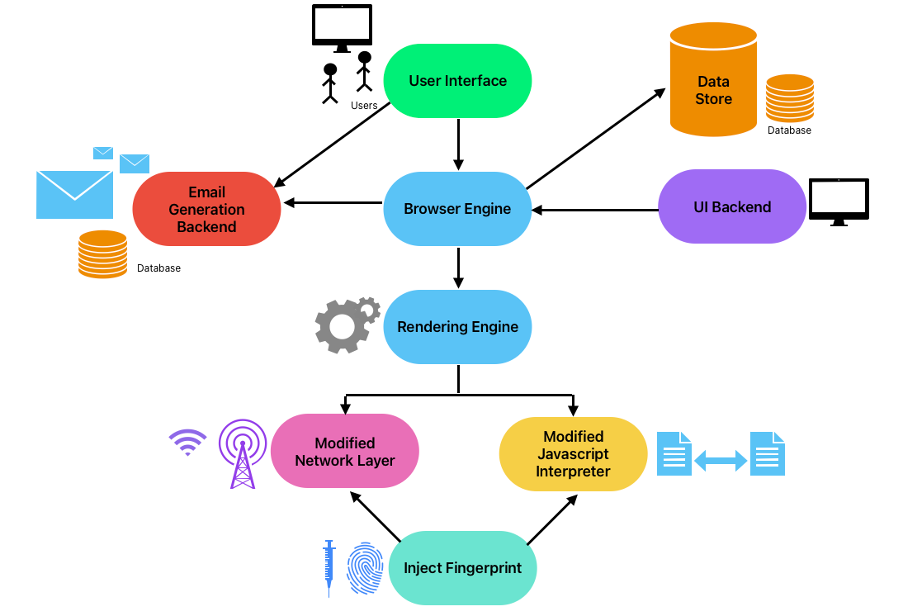
\includegraphics[width=1\linewidth]{HighLevelArch.png}}
% \caption{High Level Architecture}
% \label{fig}
% \end{figure}


% The User interface is responsible for the visual elements that you see in a browser excluding the UI of the website that is visited. It includes the maximize and minimize, bookmarks, search history, exit browser, forward and back button, refresh, and themes for light and dark mode. This is connected to the Email Generation Backend and the Browser Engine. The Browser Engine is responsible for managing the core browser operations. This component interacts with the data store, UI backend and rendering engine implemented using CefSharp which determines the speed with which the engine loads website content. The Rendering Engine implements anti-fingerprinting techniques through custom scripts and network layer modifications, safeguarding user data from tracking attempts. The modified network layer is integrated into the rendering engine and it carries injected fingerprints of the user that is transmitted using TLS and HTTP. The Normal JS Interpreter is modified for our convenience, to Interpret JS files that override attributes of fields in a fingerprint like WebGL, canvas, and other fields. The Email Generation Backend generates temporary emails for each profile. A user may sign up using any email to which all emails sent to @pryguard.org are routed for that profile. The user must approve a verification for the email routing. We used Cloudflare to rent a domain pryguard.org and set a limit on the number of emails that a user may generate at a time by each profile to prevent malicious use. These emails are used to preserve user anonymity and may be discarded by the user when desired.

% The Cookie Containerization feature enhances the browser's cookie management system to securely store first-party cookies, preventing third-party access and tracking while browsing. It involves storing data for each profile in a separate container i.e containerization of cookies is done on a per profile basis. Cookies are stored in files on the browser for each profile for every website that we query.

% PryGuard integrates a suite of randomized anti-fingerprinting techniques to create a unique and dynamic browsing footprint for each user, effectively countering tracking mechanisms that rely on device and behavioral consistency. To safeguard IP privacy, WebRTC masking substitutes local IP addresses with randomized ones, while canvas fingerprinting protection randomizes graphic rendering data to obscure hardware-specific information. PryGuard’s WebGL and audio context protection similarly inject noise and subtle variations into rendering and audio frequency data, thwarting tracking based on graphics and audio processing traits. The browser further standardizes font availability and restricts plugin visibility, minimizing tracking potential through unique font and plugin combinations. By isolating cookies per profile, PryGuard ensures that sessions remain private, blocking cross-site tracking attempts. Proxy management and IP masking offer additional anonymity by routing traffic through selectable proxies on a per-session basis. For seamless anonymous interactions online, PryGuard generates temporary email addresses using the Cloudflare API, protecting users from spam and avoiding personal data exposure. The browser also obfuscates key device properties like memory, CPU cores, battery level, and network status to further prevent tracking based on hardware resources or connection stability. Additional privacy measures include enforcing a "Do Not Track" (DNT) setting and ensuring iframe content abides by cross-origin protection rules. By using generically randomized outputs across these protections, PryGuard provides an unpredictable and resilient layer of privacy, making users' browsing patterns challenging to track and uniquely secure.

% PryGuard browser offers a robust privacy framework through multi-layered anti-fingerprinting, containerized cookie management, and randomized data injections that mask user identity and browsing behavior. By integrating temporary email generation, proxy management, and WebRTC masking, PryGuard ensures anonymity and secure online interactions. This privacy-first approach makes PryGuard a comprehensive solution to mitigate tracking and safeguard user data across the web.

% \section{Implementation}
% The design of PryGuard revolves around two core principles: privacy by design and scalability. PryGuard’s user interface is built using Windows Presentation Framework (WPF), which offers powerful data-binding capabilities. By employing the Model-View-ViewModel (MVVM) pattern, we ensure that the UI remains decoupled from the business logic. This structure enhances maintainability and scalability, allowing the browser to evolve and accommodate new privacy features without overhauling the entire system. WPF was chosen for its robust UI capabilities and seamless integration with the MVVM architecture. Compared to other frameworks, it offers better support for rich data binding, responsive layouts, themes and customization, which are essential for a browser with multiple privacy-related features like profile customization, fingerprint injection, and cookie management.
% PryGuard uses CEFSharp (Chromium Embedded Framework) at its core for rendering web pages. CEFSharp allows us to implement deep privacy controls such as anti-fingerprinting, proxy management, and cookie containerization while maintaining full compatibility with modern web technologies.
% % \begin{figure}[htbp]
% % \centerline{\includegraphics[width=1\linewidth]{image.png}}
% % \caption{Deployment Diagram}
% % \label{fig}
% % \end{figure}

% \subsection{Anti-Fingerprinting}
% The UI layer of PryGuard allows customizable user attributes by injecting new fingerprints for each profile, including user-agent, operating system version, screen resolution, canvas, WebRTC settings, geolocation, and proxy management. Proxy integration enhances anonymity, supporting HTTP, SOCKS4, and SOCKS5 protocols. Additional features like canvas hiding and user-agent/system attribute randomization provide protection against tracking techniques.

% \subsubsection{User-Agent Injection}
% The User-Agent string provides information about the browser, operating system, and device type, which websites use to identify unique users. By randomizing the User-Agent string for each profile, it becomes more challenging for websites to track the same user across sessions. The algorithm for this process involves loading a pre-configured list of commonly used User-Agent strings. For each profile, a User-Agent string is randomly selected from this list, which is then applied to the current browsing session.

% \subsubsection{Canvas Fingerprint Injection}
% Canvas fingerprinting uses the rendering of a blank HTML canvas to extract unique data based on a device’s graphics hardware and software. To obscure this data and prevent fingerprinting, PryGuard injects modified canvas output. This is achieved by creating an HTML canvas element and ensuring that when the canvas data is requested, modified image data is returned instead of the original.

% \subsubsection{WebRTC IP Leak Prevention}
% WebRTC can potentially expose the user's real IP address, even if they are using a VPN or proxy. To prevent this leakage, the algorithm accesses WebRTC settings and disables IP leakage functions, ensuring that WebRTC only uses the IP provided by the configured proxy or VPN.

% \subsubsection{Proxy Management}
% Users may select between no proxy, a new proxy that can be manually entered, or saved proxy settings that are imported from other profiles on PryGuard. This flexibility allows for enhanced anonymity by masking the user's IP address and routing traffic through different proxy servers. The algorithm retrieves the user’s preferred proxy settings and, based on their selection, configures the browser to route traffic through the specified proxy server while ensuring that fingerprinting prevention settings align with the IP and other characteristics provided by the proxy to maintain consistency.

% \subsubsection{Geolocation Injection}
% Websites can request the user’s geographical location. PryGuard sets location based on IP so that the time based anomaly is eliminated.
% The algorithm states that when a website requests location data, it must return the location based on IP.


% \subsubsection{Operating System, Screen Resolution, and Media Device Injection}
% Tracking can occur by detecting the operating system version and screen resolution of a device, which can often uniquely identify a user’s setup. To enhance anonymity, PryGuard randomizes this data. The algorithm involves loading lists of common operating system versions, screen resolutions, and media device configurations. For each user profile, an operating system version and screen resolution are randomly assigned from the respective lists, along with a media device configuration that masks the real devices connected to the user's system. These randomized values are then injected into the browser profile’s settings to prevent tracking based on system details.

% These combined techniques, when applied to each browsing profile, provide strong resistance against tracking by injecting random data for key browser and device attributes. By rotating fingerprints and using proxies, PryGuard prevents websites from creating a stable tracking profile, enhancing user privacy across browsing sessions.

% \subsection{Cookie Containerization}
% Cookie Containerization aims at isolating cookies within each profile. Profile-specific cookie storage creates and manages a unique cookie container for each profile. Session persistence retains cookies between sessions for each profile, ensuring independent tracking. The UI layer enables users to set custom cookie policies for each profile, ensuring privacy across sessions and preventing cross-site tracking, offering a significant improvement over traditional cookie management systems. For each profile, a separate container is created to store cookies. During a session, cookies are loaded from the container and saved at the end of the session, while stored cookies are maintained in local storage after the session ends. Future sessions retrieve cookies based on the profile ID.

% \subsection{Temporary Email Generation}
% PryGuard offers its users disposable email addresses for anonymous registration, managed via PryGuard’s integration with Cloudflare. Users can register on PryGuard’s website, pryguard.org, verify their identity via email, and manage temporary email addresses. PryGuard integrates with Cloudflare’s API to automate the creation of temporary email addresses linked to user profiles. The UI layer allows users to create, view, and delete temporary emails, while backend services manage email creation and routing, linking profiles with generated addresses via Cloudflare's API and storing email data in MongoDB. Users may generate up to five temporary email addresses, which they can delete at any time. This functionality prevents malicious activity and ensures privacy and anonymity by preventing email tracking. When a user registers on pryguard.org, they receive a verification email. Upon verification, email routing is set up to direct emails to the user’s primary inbox. If the user has fewer than five temporary emails, they can call the Cloudflare API to generate a new temporary email, which is stored in MongoDB with routing rules to forward emails from the temporary address to the user's verified email. Users may also call the Cloudflare API to remove the routing rule and delete the temporary email, along with its database entry.

% \subsection{Developer Tools}
% PryGuard includes developer tools to enhance usability by providing users with options like inspecting elements to view page source, debugging scripts with a console for debugging JavaScript on web pages, and a performance analyzer that allows tracking of resource usage, network requests, and memory allocation.

% \subsection{Browser UI – Search History, Downloads, Bookmarks, and Themes}
% PryGuard keeps track of and allows users to manage their search history. Users can download files, audio, and video, saving them in a desired location. Additionally, users may save and manage bookmarks for quick access and can choose between light or dark themes for the browser.

\section{Results}
The PryGuard browser emerges as a remarkable alternative in the privacy-centric browsing space, effectively competing with well-known browsers like Google Chrome, Mozilla Firefox, and Tor Browser. To evaluate performance in an isolated environment, we used Sandboxie to sandbox each browser. PryGuard provides an outstanding balance of privacy and efficiency, as shown in Table 1, which presents a detailed comparison of performance analysis highlighting PryGuard’s efficiency.

\begin{table}[h]
\centering
\caption{Performance Analysis}
\begin{tabular}{|l|c|c|c|}
\hline
Browser            & Memory Usage & CPU Usage & Page Load Time \\ \hline
PryGuard          & 277.0 MB     & 0.1\%     & 1511 ms         \\ \hline
Google Chrome     & 567.2 MB     & 0.2\%     & 1807 ms         \\ \hline
Tor Browser       & 671.6 MB     & 0.1\%     & 7950 ms         \\ \hline
Mozilla Firefox    & 503.5 MB     & 0.1\%     & 1297 ms         \\ \hline
\end{tabular}
\end{table}

PryGuard stands out due to its superior privacy protection which actively protects against tracking techniques through fingerprint injection, cookie containerization, proxy management and temporary email generation, maintaining user anonymity. It is designed to prevent websites from identifying users based on their device and browser characteristics. PryGuard successfully meets the standard of IPHey browser fingerprinting which assures that our browser is trustworthy. PryGuard portrays balanced efficiency by achieving exceptional performance compared to leading browsers in memory and CPU while maintaining advanced privacy. PryGuard is designed for users to enjoy online freedom by allowing them to control their digital footprint, and providing comprehensive protection without heavy resource use.

\section{Conclusion}
PryGuard addresses the critical need for a privacy-focused browser capable of countering advanced tracking techniques with remarkable efficiency. Through innovative features such as fingerprint injection, cookie containerization, proxy management, and temporary email generation, PryGuard offers a comprehensive solution for users concerned about online privacy. With its unique balance of speed, privacy, and low resource usage, PryGuard is a next-generation browser for users who prioritize both privacy and performance, proving itself as an exceptional alternative to mainstream options. The results of extensive testing demonstrate that PryGuard not only enhances privacy protection but also maintains high performance, making it a viable alternative to mainstream browsers.

\section{Future Work}
Future enhancements to PryGuard may include implementing additional privacy features like Browser Extensions Support, allowing users to integrate existing privacy-focused extensions seamlessly into PryGuard. Fine grained cookie containerisation, i.e. containerisation of each website for every profile to prevent leakage of cookies. Scaling of the email generation with Cloudflare API integration may be explored further, focusing on managing email limits. Enable email routing specifically to PryGuard users. Include more hardware-based fingerprint injection techniques to make the anti-fingerprinting feature complete and secure. Integration of VPN Services providing users with an option to route all browser traffic through a secure VPN, enhancing anonymity further. Further Optimization of Performance by continually refining the codebase to improve speed and resource management.
\end{itemize}



\begin{thebibliography}{00}
\bibitem{b1} Pierre Laperdrix, Nataliia Bielova, Benoit Baudry, and Gildas Avoine. "Browser Fingerprinting: A Survey." \textit{ACM Transactions on the Web}, vol. 14, no. 2, Article 8, May 2020, pp. 33. \url{https://doi.org/10.1145/3386040}

\bibitem{b2} H. Hu, P. Peng, and G. Wang. "Characterizing Pixel Tracking through the Lens of Disposable Email Services." \textit{2019 IEEE Symposium on Security and Privacy (SP)}, San Francisco, CA, USA, 2019, pp. 365–379. \url{https://doi.org/10.1109/SP.2019.00033}

\bibitem{b3} V. L. Ajay and A. M. Guptha. "A Defense against JavaScript Object-Based Fingerprinting and Passive Fingerprinting." \textit{2022 International Conference on Computing, Communication, Security and Intelligent Systems (IC3SIS)}, Kochi, India, 2022, pp. 1–6. \url{https://doi.org/10.1109/IC3SIS54991.2022.9885716}

\bibitem{b4} Jianhui Zhang, Youjun Bu, Bo Chen, Chongxin Sun, and Tianyu Wang. "A Survey of Browser Fingerprint Research and Application." \textit{Security and Communication Networks}, 2022, Article ID 3363335, pp. 14. \url{https://doi.org/10.1155/2022/3363335}

\bibitem{b5} T. Li, X. Zheng, K. Shen, and X. Han. "FPFlow: Detect and Prevent Browser Fingerprinting with Dynamic Taint Analysis." In: Lu, W., Zhang, Y., Wen, W., Yan, H., Li, C. (eds). \textit{Cyber Security, CNCERT 2021}, Communications in Computer and Information Science, vol. 1506, Springer, Singapore, 2022, pp. 60–77. \url{https://doi.org/10.1007/978-981-16-9229-1\_4}

\bibitem{b6} N. Mathews, J. K. Holland, S. E. Oh, M. S. Rahman, N. Hopper, and M. Wright. "SoK: A Critical Evaluation of Efficient Website Fingerprinting Defenses." \textit{2023 IEEE Symposium on Security and Privacy (SP)}, San Francisco, CA, USA, 2023, pp. 969–986. \url{https://ieeexplore.ieee.org/abstract/document/10179289}

\bibitem{b7} Babak Amin Azad, Oleksii Starov, Pierre Laperdrix, and Nick Nikiforakis. "Taming the Shape Shifter: Detecting Anti-fingerprinting Browsers." \textit{DIMVA 2020 - 17th Conference on Detection of Intrusions and Malware \& Vulnerability Assessment}, Lisboa / Virtual, Portugal, Jun 2020, pp. 10. \url{https://www.securitee.org/files/antifpbrowsers\_dimva2020.pdf}

\end{thebibliography}



\vspace{12pt}


\end{document}
